\section {The Arduino implementation of SOS protocol}
\begin{frame} {Outline}
    \tableofcontents [current]
\end{frame}

\begin{frame}[containsverbatim]{SOS usage}
	\begin{columns}[c]
		\begin{column}[c]{.6\textwidth}
\begin{Verbatim}[fontsize=\scriptsize]
void setup() 
{
  sos = new Sos(mac_addr, 123);
  // it will change
  sos->register_resource(
    "temp",
    "Temperature",
    "temp",
    handler);
}
\end{Verbatim}
		\end{column}
		\begin{column}[c]{.4\textwidth}
\begin{Verbatim}[fontsize=\scriptsize]
void loop() 
{
  sos->loop();
}
\end{Verbatim}
		\end{column}
	\end{columns}
\end{frame}

\begin{frame}[containsverbatim]{resistor and led}
	\begin{columns}[c,onlytextwidth]
		\begin{column}[c]{.5\textwidth}
			\begin{center}
				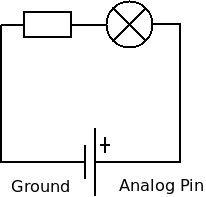
\includegraphics [width=.9\textwidth,keepaspectratio]{img/resistor_led_analog.png}
			\end{center}
		\end{column}
		\begin{column}[c]{.5\textwidth}
\begin{Verbatim}[fontsize=\scriptsize]
uint8_t process_led(Message &in, 
	               Message &out) 
{
  int n;
  for(option * o = in.get_option() ; 
    o != NULL ; o = in.get_option())
  {
    if(o->optcode() == option::MO_Uri_Query)
    {
      if(sscanf ((const char *) opt.val(), 
          "val=%d", &n) == 1)
      	analogWrite(led, n);
      out.set_code(COAP_RETURN_CODE(2,5));
    }
  }
  return 0;
}
\end{Verbatim}
		\end{column}
	\end{columns}
\end{frame}

\begin{frame}[containsverbatim]{resistor and photoresistor}
	\begin{columns}[c,onlytextwidth]
		\begin{column}[c]{.5\textwidth}
			\begin{center}
				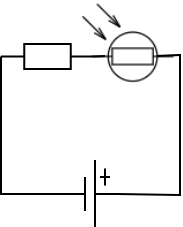
\includegraphics [width=.9\textwidth,keepaspectratio]{img/resistor_photoresistor.png}
			\end{center}
		\end{column}
		\begin{column}[c]{.5\textwidth}
\begin{Verbatim}[fontsize=\scriptsize]
uint8_t process_light(Message &in, 
                     Message &out) 
{
  char message[10];
  for(int i(0) ; i < 10 ; i++)
    message[i] = '\0';
  int sensorValue = 
    analogRead(light_sensor);
  snprintf(message, 10, "%d\0", 
                  sensorValue);
  out.set_payload( strlen(message), 
        (unsigned char *) message);
  out.set_code(COAP_RETURN_CODE(2,5));
  return 0;
}
\end{Verbatim}
		\end{column}
	\end{columns}
\end{frame}

\begin{frame}{Stats}
	\begin{center}
		\includegraphics<1> [width=1\textwidth,keepaspectratio] {pdf/memory0.pdf}
		\includegraphics<2> [width=1\textwidth,keepaspectratio] {pdf/memory1.pdf}
	\end{center}
\end{frame}

\begin{frame} {W5100}
	\begin{itemize}
		\item One position possible on the Arduino
		\item Runs on 3 modes : 
		\begin{itemize}
			\item UDP
			\item TCP
			\item MAC Raw
		\end{itemize}
		\item Advantage : simple to work with UDP and TCP
		\item Inconvenient : need to implement all other protocols
	\end{itemize}
\end{frame}

\begin{frame} {Difficulties}
    \begin{itemize}
		\item SRAM = 2Ko
		\item W5100 : easy in UDP and TCP mode, less in MAC Raw
		\item no debug facility
		\begin{itemize}
			\item no gdb, no valgrind
			\item when the program reboots : no warning message
		\end{itemize}
		\item packet loss on busy network
    \end{itemize}
\end{frame}


